\section{Introduction}

% Example references: \cite{2015arXiv150907408D}, \citep{2016arXiv160600393K}, and \cite{tevcat}.

%  \begin{figure}[tb]
%    \centerline{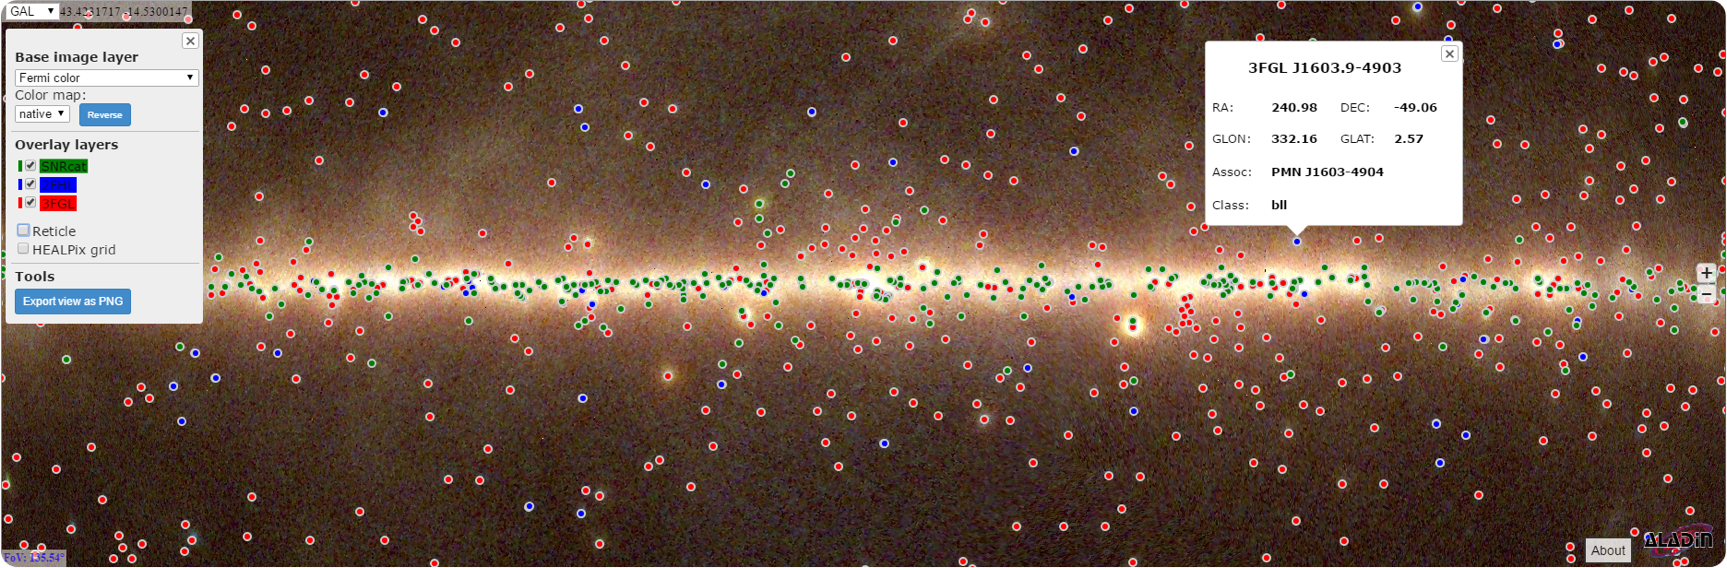
\includegraphics[width=\textwidth]{figures/fig1}}
%    \caption{Example Figure.}
%  \end{figure}
%
%  % Table
\begin{table}[h]

\caption{Example table}
\label{tab:a}
\tabcolsep7pt\begin{tabular}{lcccc}
\hline
  & \tch{1}{c}{b}{Single\\ outlet}  & \tch{1}{c}{b}{Small\\ multiple\tabnoteref{t1n1}}  & \tch{1}{c}{b}{Large\\ multiple}  & \tch{1}{c}{b}{Total}   \\
\hline
1982 & 98 & 129 & 620    & 847\\
1987 & 138 & 176 & 1000  & 1314\\
1991 & 173 & 248 & 1230  & 1651\\
1998 & 200 & 300 & 1500\tabnoteref{t1n2}  & 2000\\
\hline
\end{tabular}
\tablenote[t1n1]{This is an example of first tablenote entry. This is an example of first tablenote entry.}
\tablenote[t1n2]{This is an example of second tablenote entry.}
\end{table}


\begin{itemize}

\item Evolution of VHE gamma-ray astronomy - increasing number of detections, novel Cherenkov telescope arrays (especially CTA)

\item Upcoming surveys like HGPS (by MPIK) - clearer resolution than our current surveys

\item Because of an increasing interest in the field, there is a need for a hub of VHE data (GeV, TeV) across many different catalogs.
This is what gamma-sky was created for.

\end{itemize}
